\documentclass[]{article}

\usepackage[utf8]{inputenc}
\usepackage{tikz}

\begin{document}
   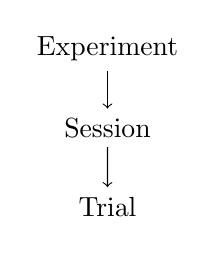
\begin{tikzpicture}[
%      align = flush center,
     grow = down,
     level distance = 1cm,
     sibling distance = 1.5cm,
     ->
    ]
   
    \node {Experiment}
     child {
      node {Session}
       child { node {Trial} }
     };
   \end{tikzpicture}


  \vspace{3cm}
   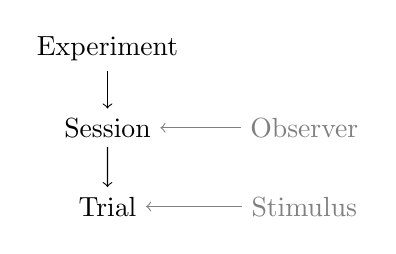
\begin{tikzpicture}[
%      align = flush center,
     grow = down,
     level distance = 1cm,
     sibling distance = 1.5cm,
     ->
    ]
   
    \node {Experiment}
     child {
      node (Session){Session}
       child { node (Trial) {Trial} }
     };
    
    \node [right of = Session, node distance = 2.5cm, gray] (Observer) {Observer}
    edge [->,  gray](Session);
    \node [right of = Trial,   node distance = 2.5cm, gray] (Stimulus) {Stimulus}
    edge [->,  gray](Trial);
   
   \end{tikzpicture}
    
   \vspace{3cm}
   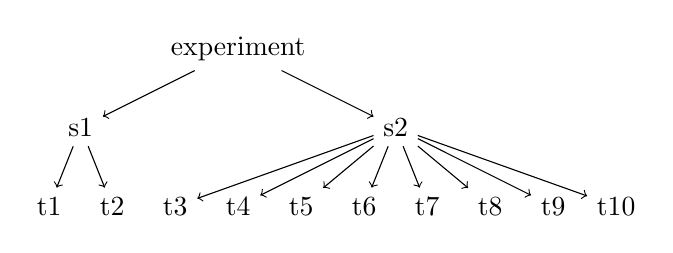
\begin{tikzpicture}[
     grow = down,
     level distance = 1cm,
     sibling distance = 1.5cm,
     ->
    ]
    \tikzstyle{level 1}=[sibling distance=4cm]
    \tikzstyle{level 2}=[sibling distance=0.8cm]
    \tikzstyle{level 3}=[sibling distance=1cm]

    \node {experiment}
     child { node {s1}
       child { node {t1} }
       child { node {t2} }
     }
     child { node {s2}
       child { node {t3} }
       child { node {t4} }
       child { node {t5} }
       child { node {t6} }
       child { node {t7} }
       child { node {t8} }
       child { node {t9} }
       child { node {t10} }
     };
   \end{tikzpicture}


   \newpage
   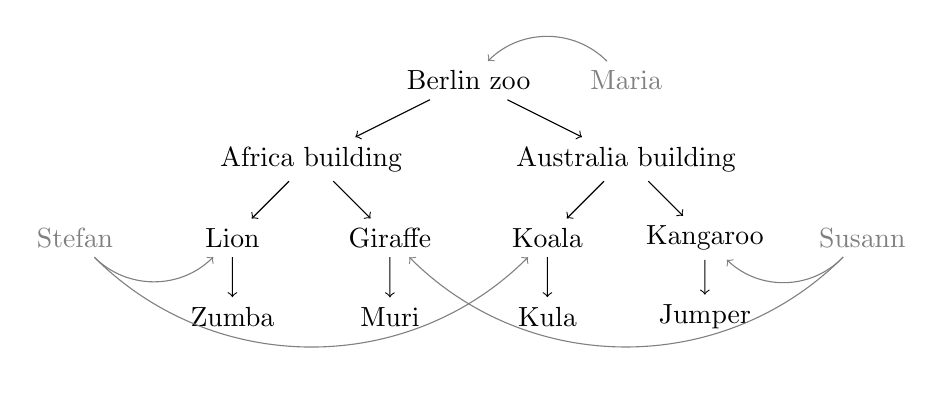
\begin{tikzpicture}[
%      align = flush center,
     grow = down,
     level distance = 1cm,
     sibling distance = 3.5cm,
     ->
    ]
   \tikzstyle{level 1}=[sibling distance=4cm]
    \tikzstyle{level 2}=[sibling distance=2cm]
    \tikzstyle{level 3}=[sibling distance=1cm]


    \node (zoo){Berlin zoo}
     child {node {Africa building}
       child { node (lion){Lion} 
        child{ node {Zumba}}
       }
       child { node (giraffe) {Giraffe}  
	child{ node {Muri}}
       }
     }
     child {node{Australia building} 
       child { node (koala){Koala} 
        child{ node {Kula}}
       }
       child { node (kangaroo) {Kangaroo} 
	child{ node {Jumper}}
       }
     };
    
    \node[right of = zoo, node distance = 2cm, gray] (Maria) {Maria}
    edge [->, bend right=45, gray](zoo);


    \node [right of = kangaroo,   node distance = 2cm, gray] (Susann) {Susann}
    edge [->,bend left=45, gray] (kangaroo)
    edge [->,bend left=45, gray] (giraffe);
    
    \node [left of = lion,   node distance = 2cm, gray] (Stefan) {Stefan}
    edge [->,bend right=45, gray] (lion)
    edge [->,bend right=45, gray] (koala);
   \end{tikzpicture}
  

    \vspace{3cm}
    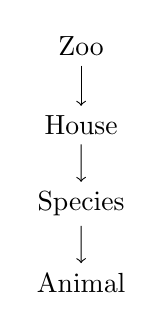
\begin{tikzpicture}[
%      align = flush center,
     grow = down,
     level distance = 1cm,
     sibling distance = 3.5cm,
     ->
    ]
    \node {Zoo}
     child { node {House}
       child { node {Species} 
	  child { node {Animal} }
       }
     };
   \end{tikzpicture}


    \vspace{3cm}
    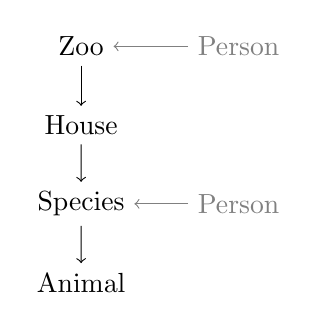
\begin{tikzpicture}[
%      align = flush center,
     grow = down,
     level distance = 1cm,
     sibling distance = 3.5cm,
     ->
    ]
    \node (zoo){Zoo}
     child { node {House}
       child { node (species){Species} 
	  child { node {Animal} }
       }
     };
    
    \node[right of = zoo, node distance = 2cm, gray] {Person}
    edge [->,  gray](zoo);

    \node[right of = species, node distance = 2cm, gray] {Person}
    edge [->,  gray](species);

   \end{tikzpicture}



\end{document}
